\documentclass[12pt]{article}
\usepackage[utf8]{inputenc}
\usepackage[greek,english]{babel}
\usepackage{alphabeta}
\usepackage{fancyhdr}
\usepackage{listings}
\usepackage{mathtools}
\usepackage{xcolor}
\usepackage{float}
\usepackage{siunitx}
\usepackage[margin=0.5in]{geometry}
\usepackage[backend=bibtex]{biblatex}

\title{Εργαστήριο Μικροηλεκτρονικής -- Εργασία 5}
\author{Χρήστος Μαργιώλης -- 19390133}
\date{Ιούνιος 2022}

\begin{document}

\begin{titlepage}
        \maketitle
        \begin{figure}[t!]
        \begin{center}
        
\includegraphics[scale=0.3]{./res/uniwalogo.png} \\
        \Large
        \textbf{Πανεπιστήμιο Δυτικής Αττικής} \\
        \large
        Τμήμα Μηχανικών Πληροφορικής και Ηλεκτρονικών Υπολογιστών
        \end{center}
        \end{figure}
\end{titlepage}

\renewcommand{\contentsname}{Περιεχόμενα}
\tableofcontents
\pagebreak

\section{Θεωρητικό μέρος}

Το αντικείμενο της εργασίας είναι η εξοικείωση και η υλοποίηση ενός ολοκληρωτή.
Ο ολοκληρωτής είναι ένα κύκλωμα το οποίο εκτελεί την μαθηματική πράξη της
ολοκλήρωσης σε ένα σήμα. 'Οσον αφορά το κύκλωμα, ο ιδανικός ολοκληρωτής είναι
ένας αναστρέφων Τ.Ε με την διαφορά ότι αντί για feedback αντίσταση υπάρχει
πυκνωτής ο οποίος έχει άεργη αντίσταση εισόδου:
\[X_c = \frac{1}{j2\pi fC}\]
Στον πρακτικό ολοκληρωτή, προκειμένου να περιορίσουμε το κέρδος του,
προσθέτουμε και μία αντίσταση ανάδρασης παράλληλα με τον πυκνωτή. Τέλος, για
συχνότητα μεγαλύτερης της $F_c$, ο ολοκληρωτής παύει να ολοκληρώνει και
συμπεριφέρεται σαν απλός αναστρέφων Τ.Ε με κέρδος:
\[-\frac{R_f}{R_{in}}\]

\section{Υλοποίηση της εργασίας}

Για την υλοποίηση της εργασίας χρησιμοποιήθηκαν τα παρακάτω εργαλεία:
\begin{itemize}
	\item Tina-TI για την συνδεσμολογία και τις μετρήσεις του κυκλώματος.
	\item Το breadboard του και τον παλμογράφο εργαστηρίου.
	\item \LaTeX για την συγγραφή της εργασίας.
\end{itemize}

\section{Συνδεσμολόγηση κυκλώματος}

\begin{itemize}
	\item Συνδεσμολογήστε το κύκλωμα με $R_{in} = R_1= \SI{10}{\kohm}$,
		$R_f = \SI{100}{\kohm}$, $C_1 = \SI{4.7}{\nano\farad}$,
		$V_1 = \SI{15}{\volt}$, $V_2 = \SI{-15}{\volt}$
\end{itemize}

\begin{figure}[H]
	\centering
	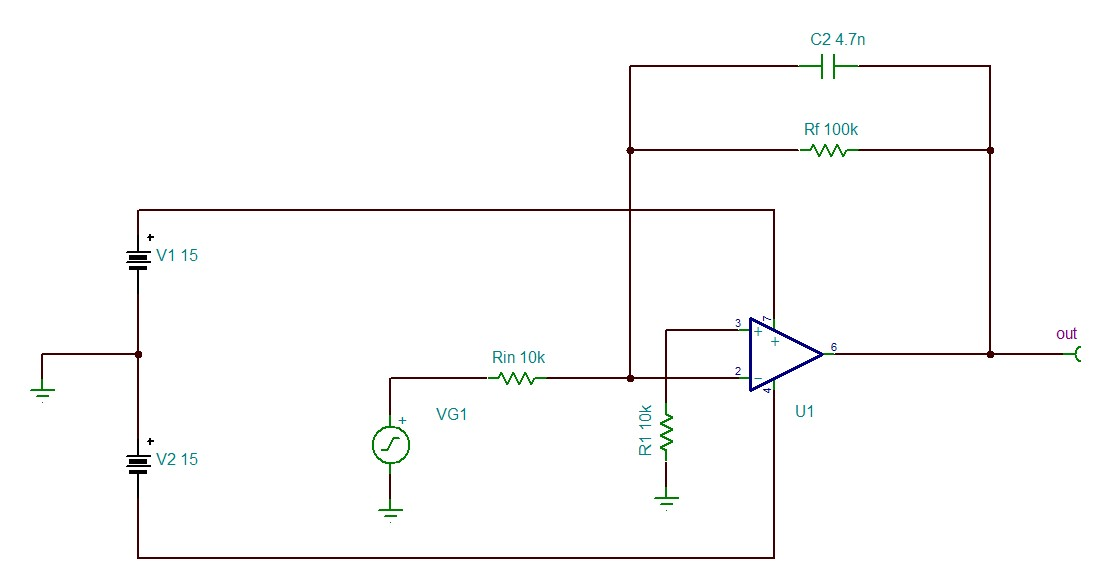
\includegraphics[width=\linewidth]{./res/schem.jpg}
	\caption{Ολοκληρωτής.}
\end{figure}

\section{Εφαρμογή σήματος}

\begin{itemize}
	\item Εφαρμόστε τριγωνική/ημιτονική/τετραγωνική κυματομορφή πλάτους
		$10V_{pp}$, $\SI{10}{\kilo\hertz}$ στην είσοδο του κυκλώματος.
\end{itemize}

\subsection{Θεωρητική $F_c$}

\begin{itemize}
	\item Υπολογίστε την θεωρητική $F_c$ του κυκλώματος.
\end{itemize}

\[F_c = \frac{1}{2 \pi R_{in} C} \Rightarrow
F_c = \frac{1}{2 \pi \cdot \SI{10}{\kohm} \cdot \SI{4.7}{\nano\farad}} \Rightarrow
F_c = \approx \SI{3.3}{\kilo\hertz}\]

\subsection{Λειτουργία $R_1$}

\begin{itemize}
	\item Ποια είναι η λειτουργία της αντίστασης $R_1$;
\end{itemize}

Δημιουργεί μετατόπιση (offset) στην έξοδο.

\subsection{Γράφημα εξόδου}

\begin{itemize}
	\item Αναπαραστήστε σε γράφημα την έξοδο του κυκλώματος ως προς την
		είσοδο για $F = \SI{10}{\kilo\hertz}$, $F >> F_c$, $F << F_c$.
\end{itemize}

\begin{figure}[H]
	\centering
	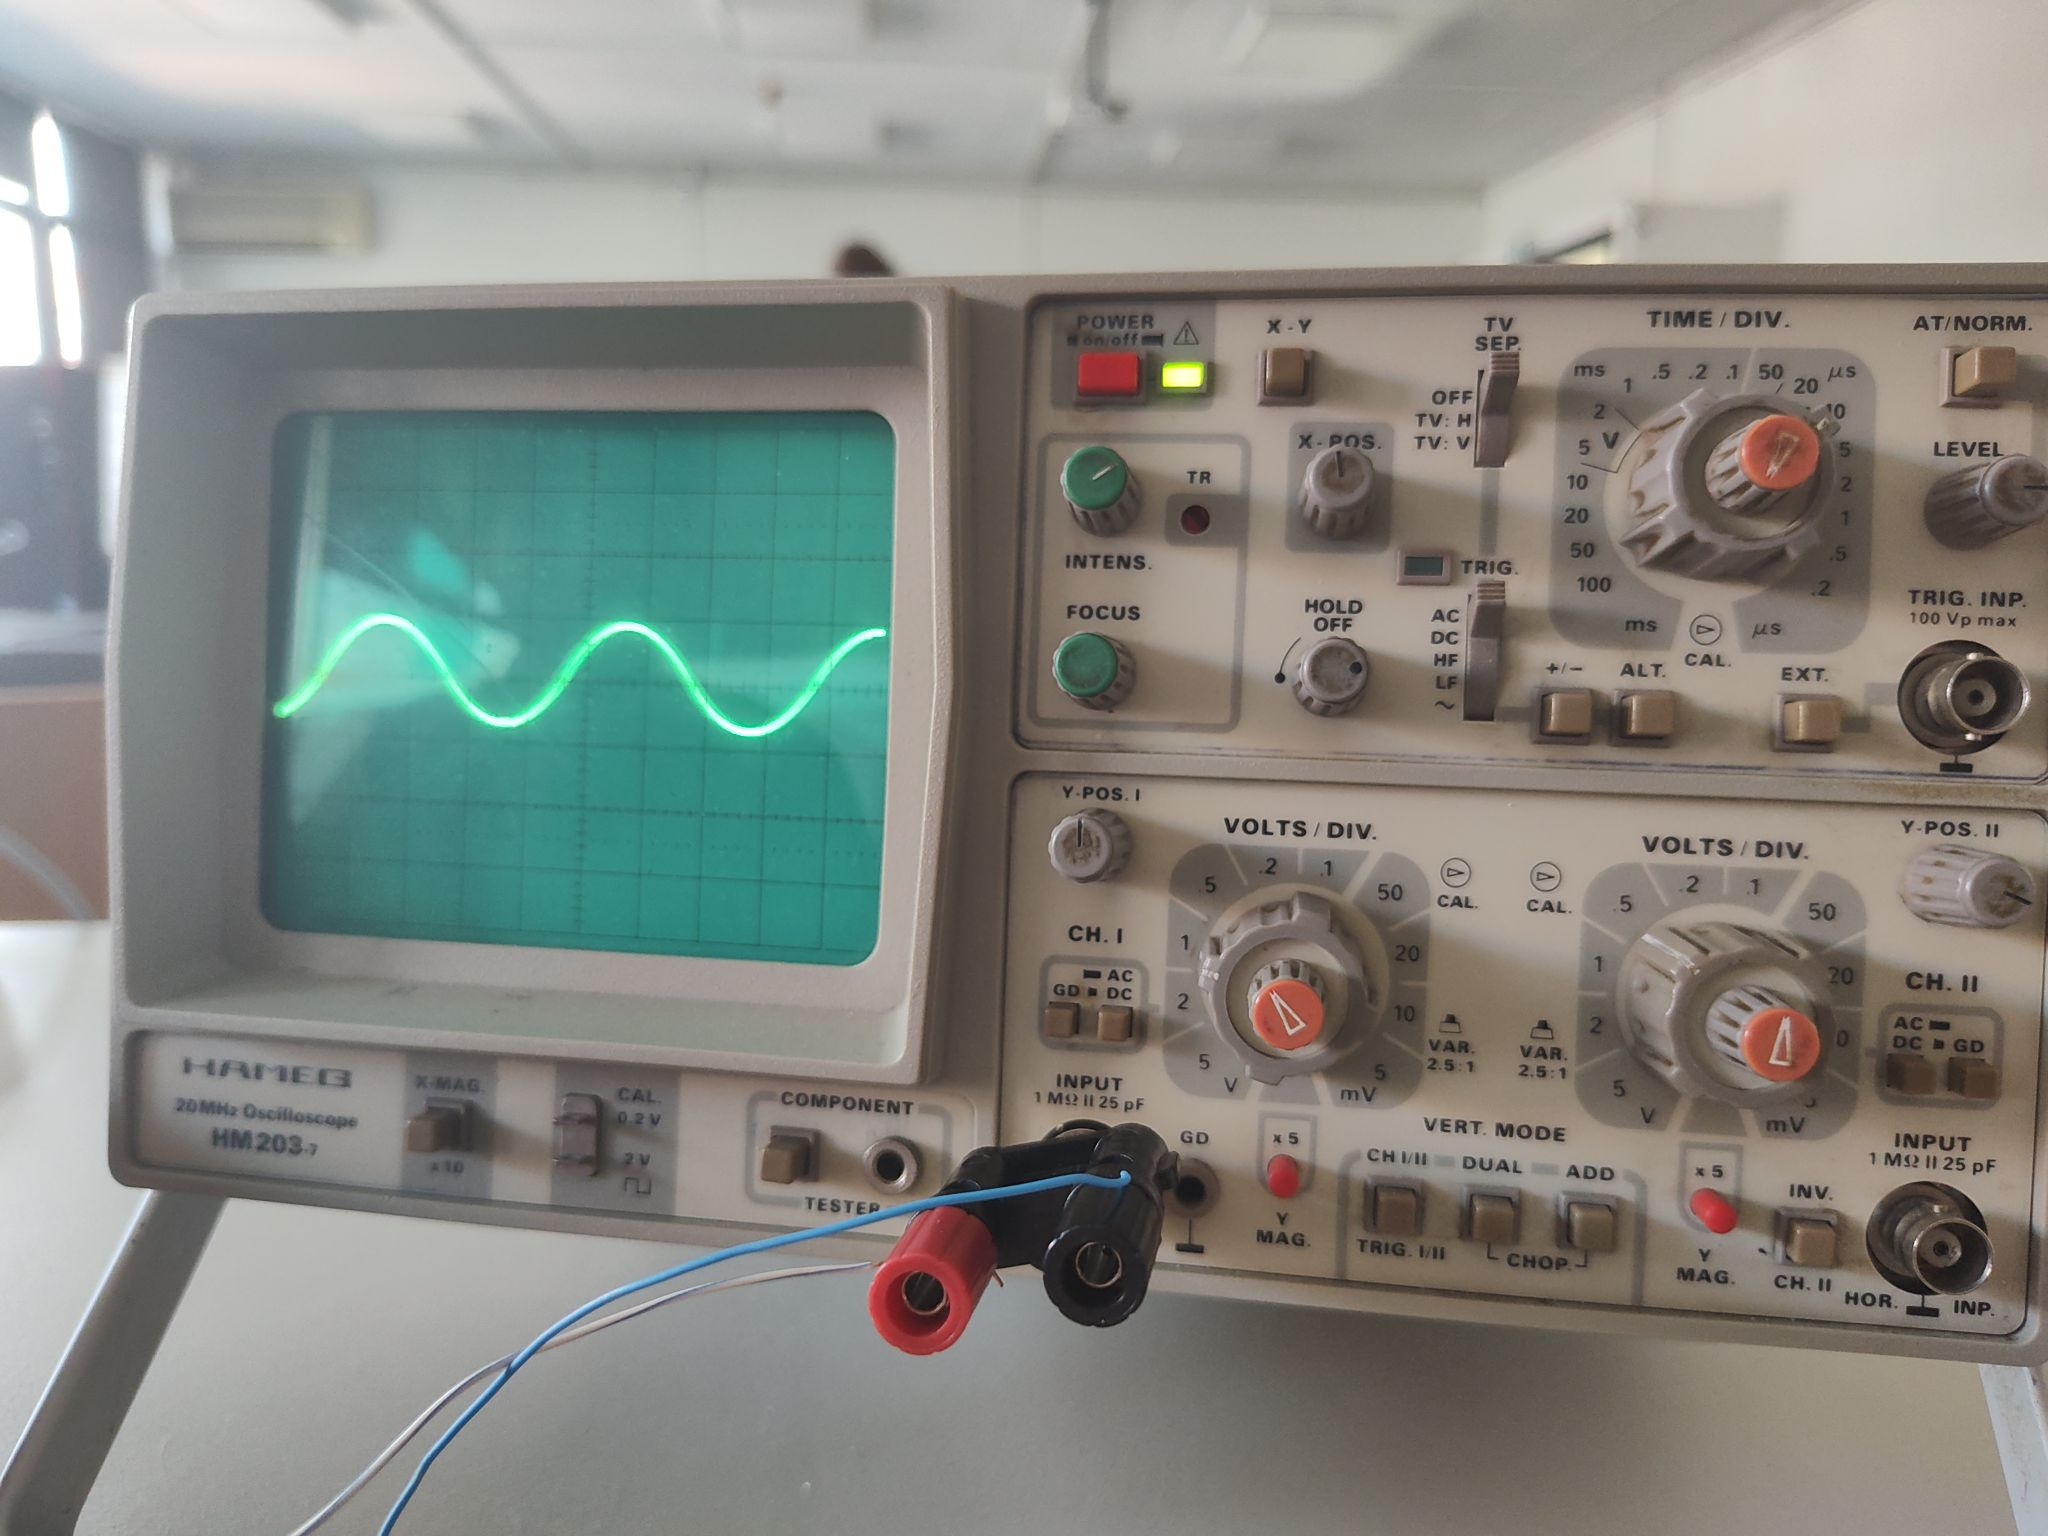
\includegraphics[width=\linewidth]{./res/sine_real.jpg}
	\caption{Ημιτονικό σήμα στον εργαστηριακό παλμογράφο.}
\end{figure}

\begin{figure}[H]
	\centering
	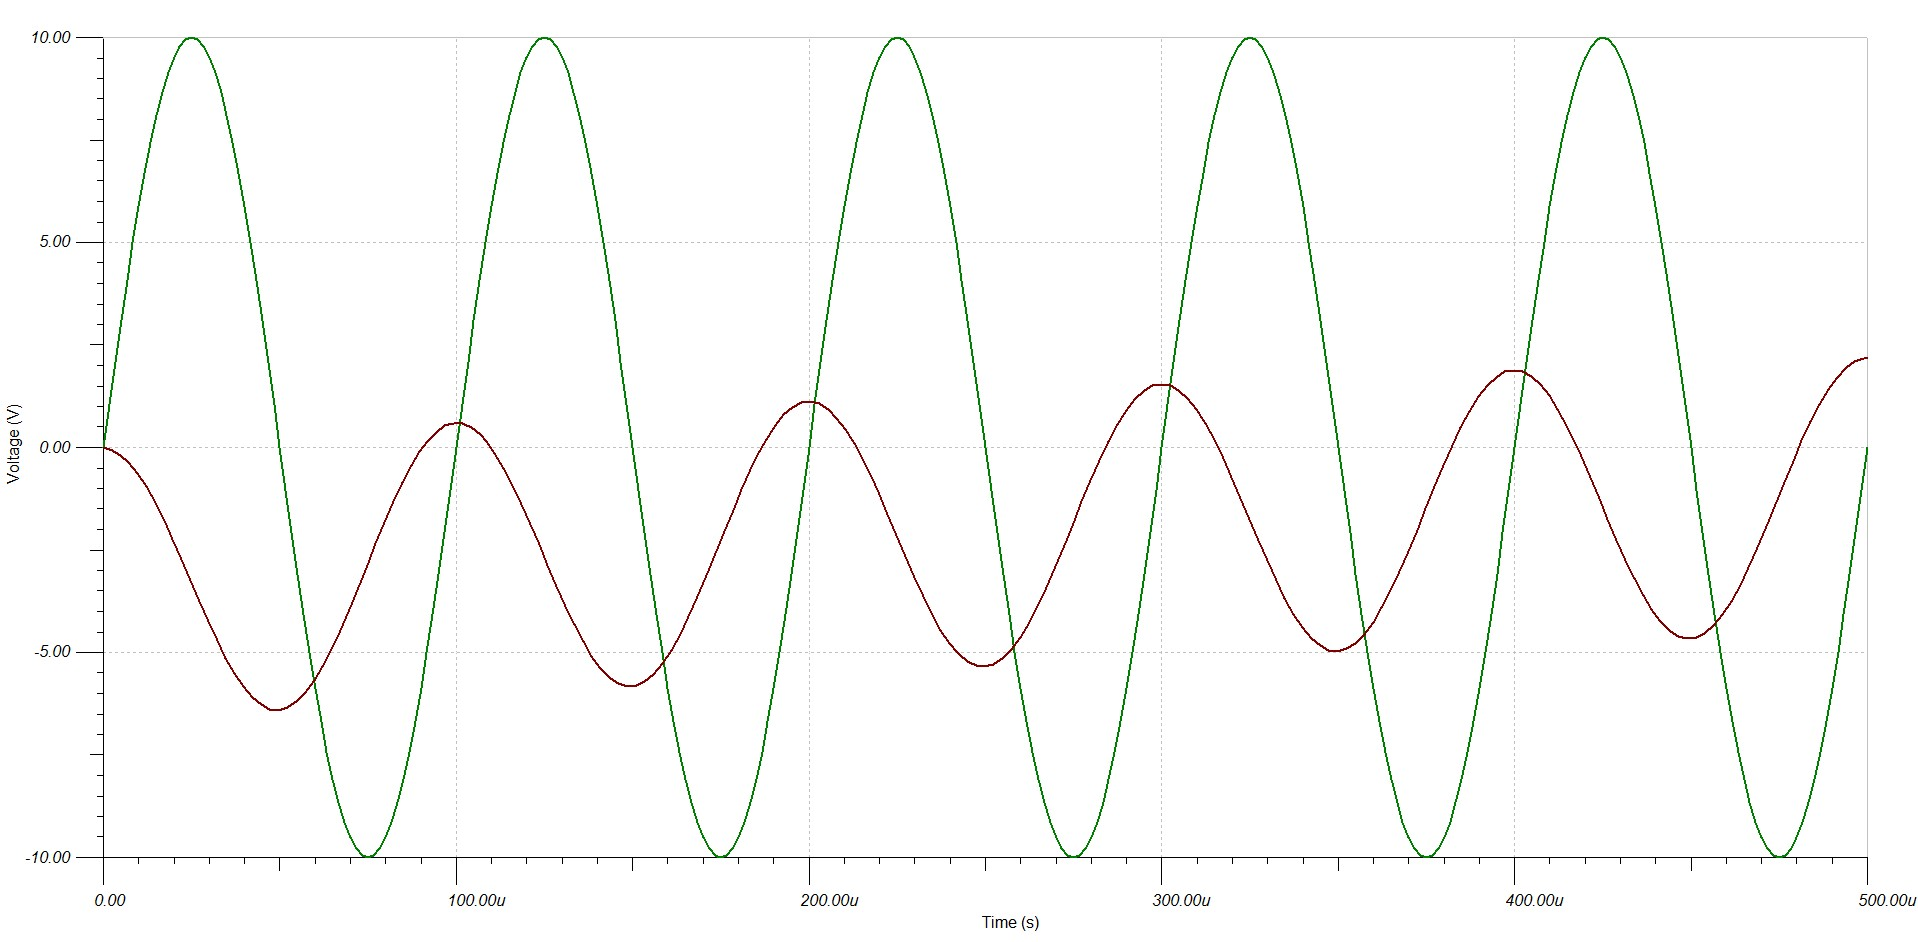
\includegraphics[width=\linewidth]{./res/sine.jpg}
	\caption{Ημιτονικό σήμα.}
\end{figure}

\begin{figure}[H]
	\centering
	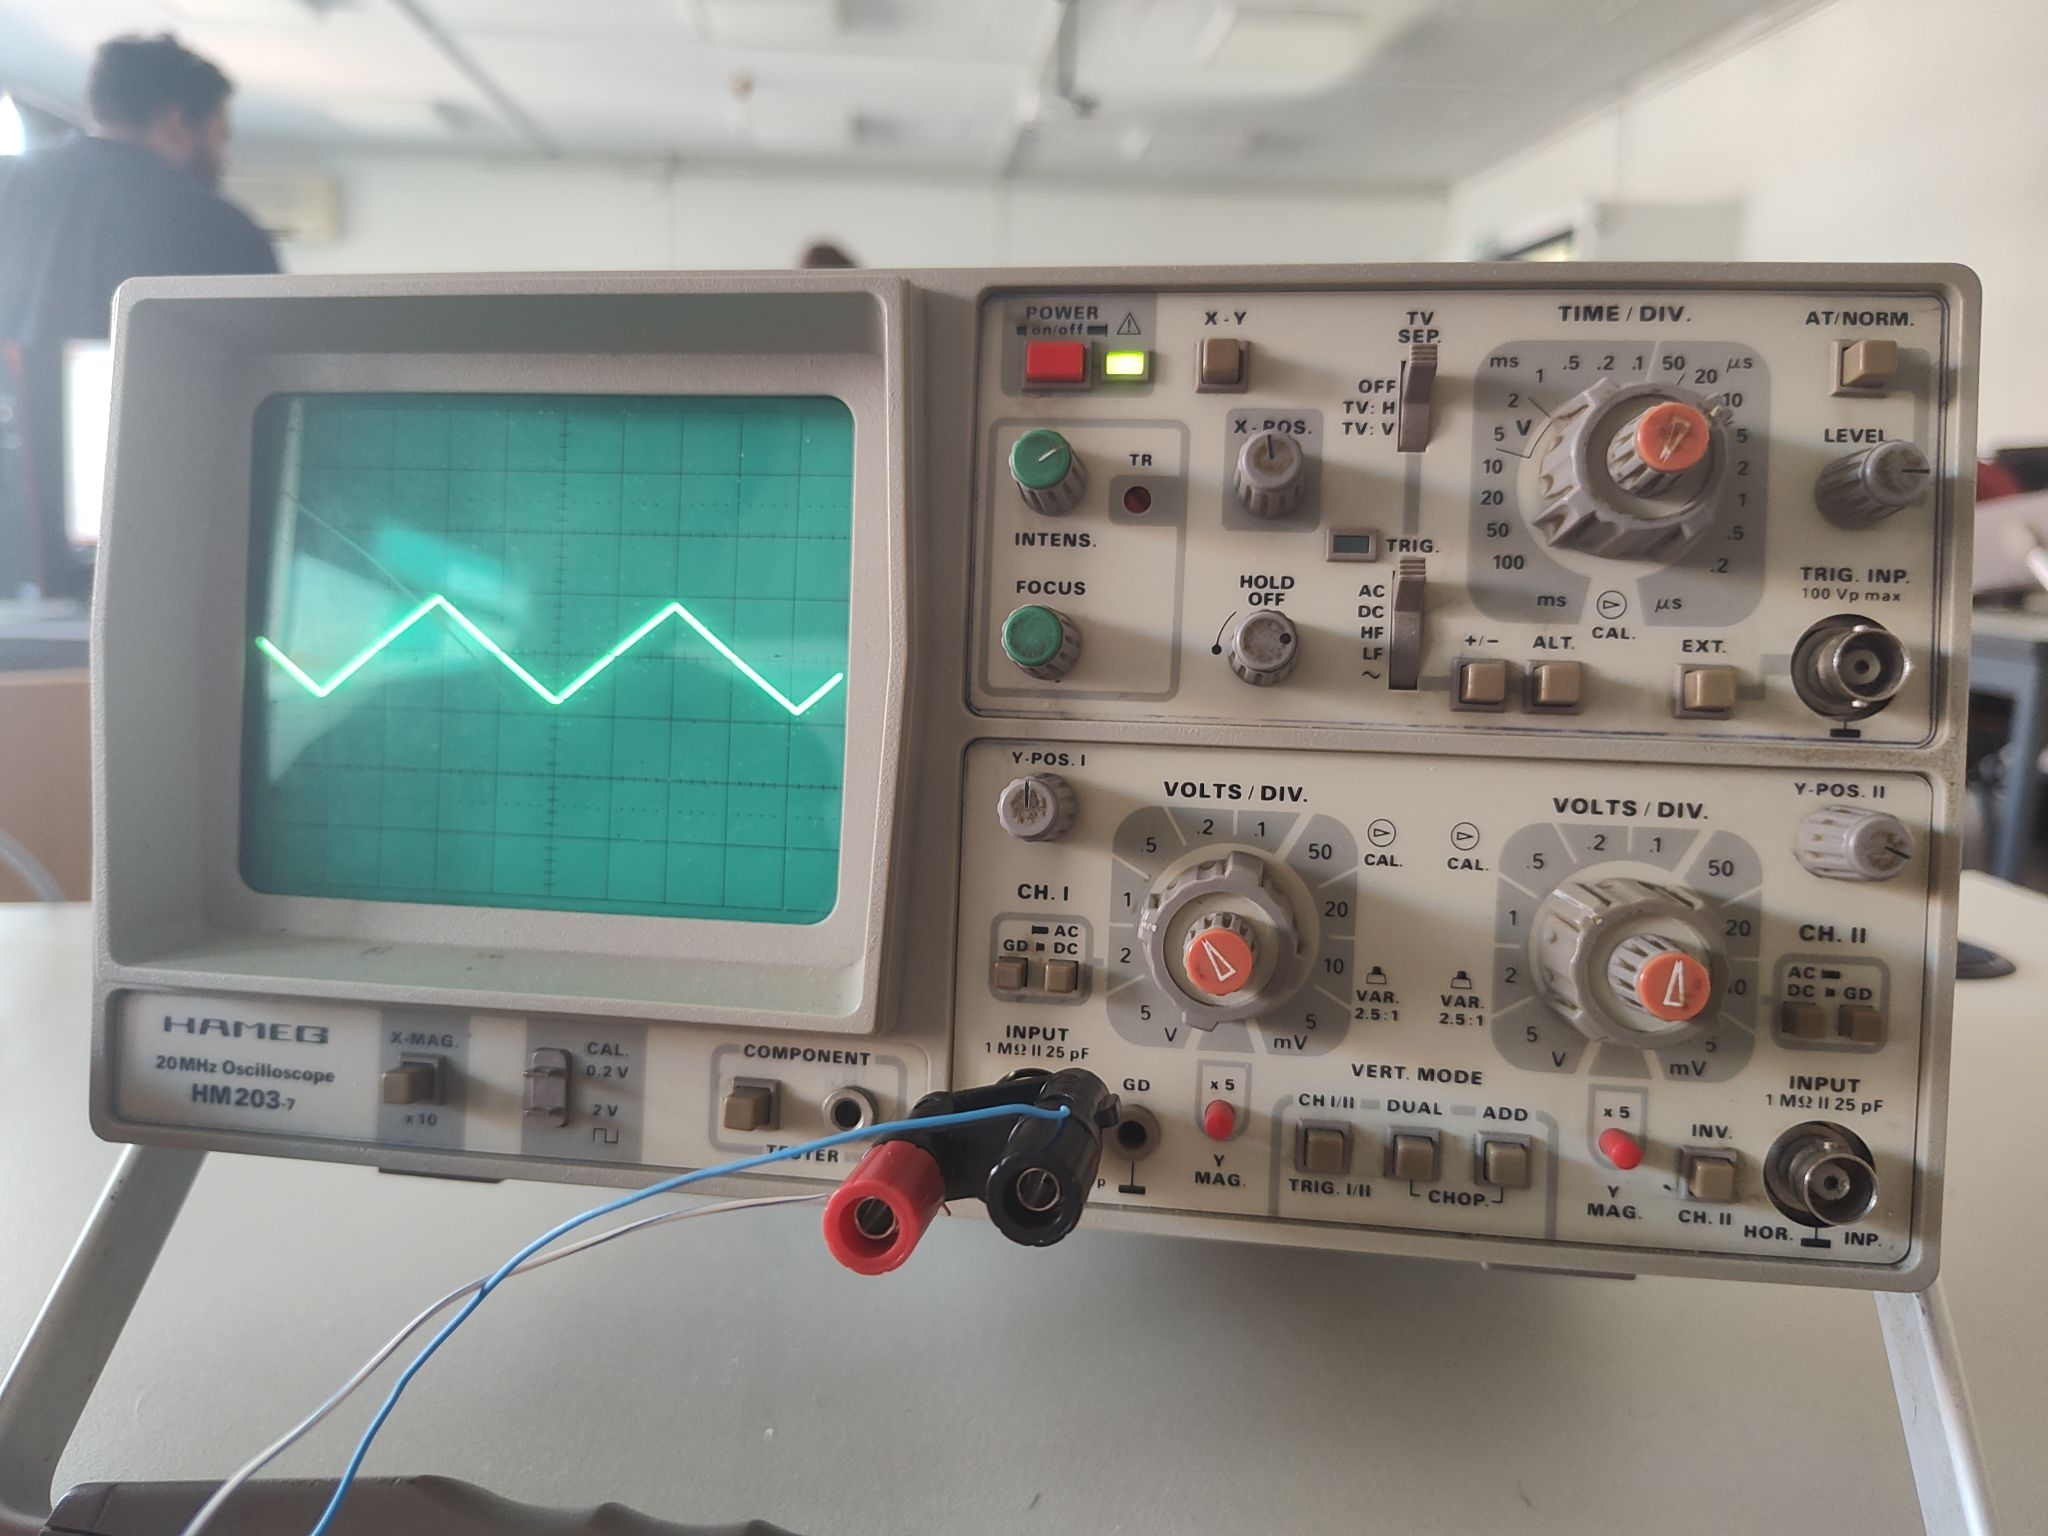
\includegraphics[width=\linewidth]{./res/triang_real.jpg}
	\caption{Τριγωνικό σήμα στον εργαστηριακό παλμογράφο.}
\end{figure}

\begin{figure}[H]
	\centering
	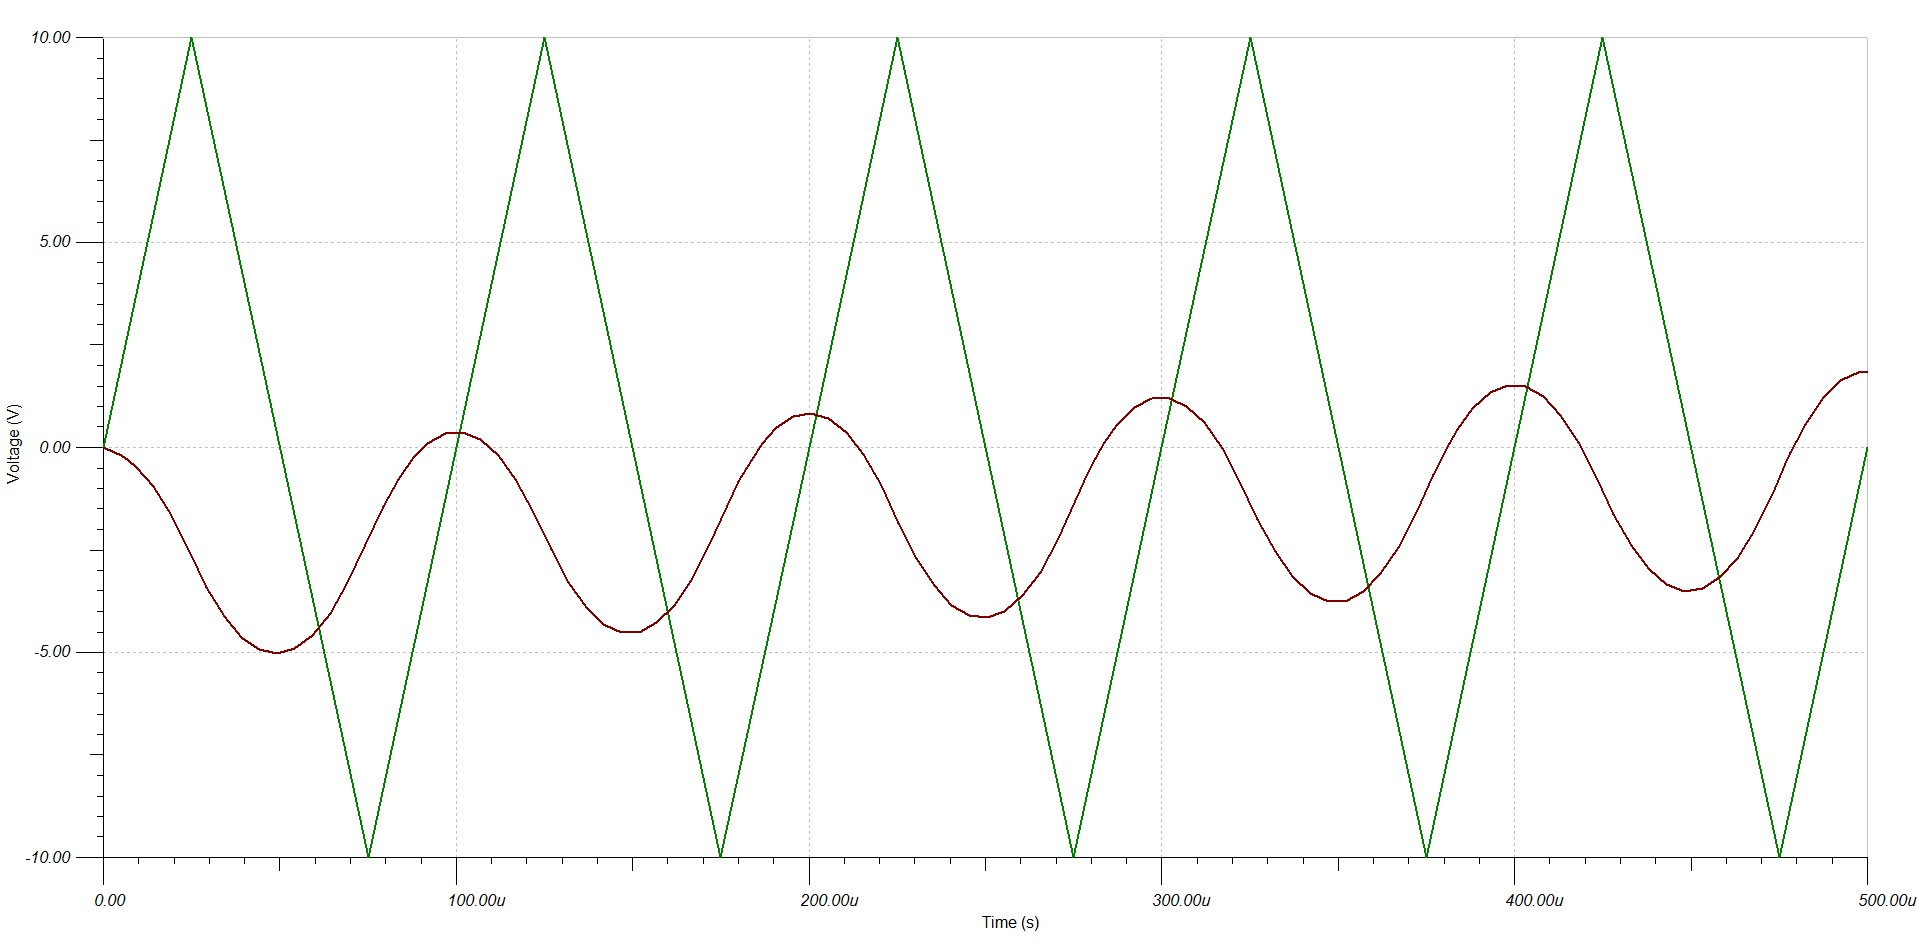
\includegraphics[width=\linewidth]{./res/triang.jpg}
	\caption{Τριγωνικό σήμα.}
\end{figure}

\begin{figure}[H]
	\centering
	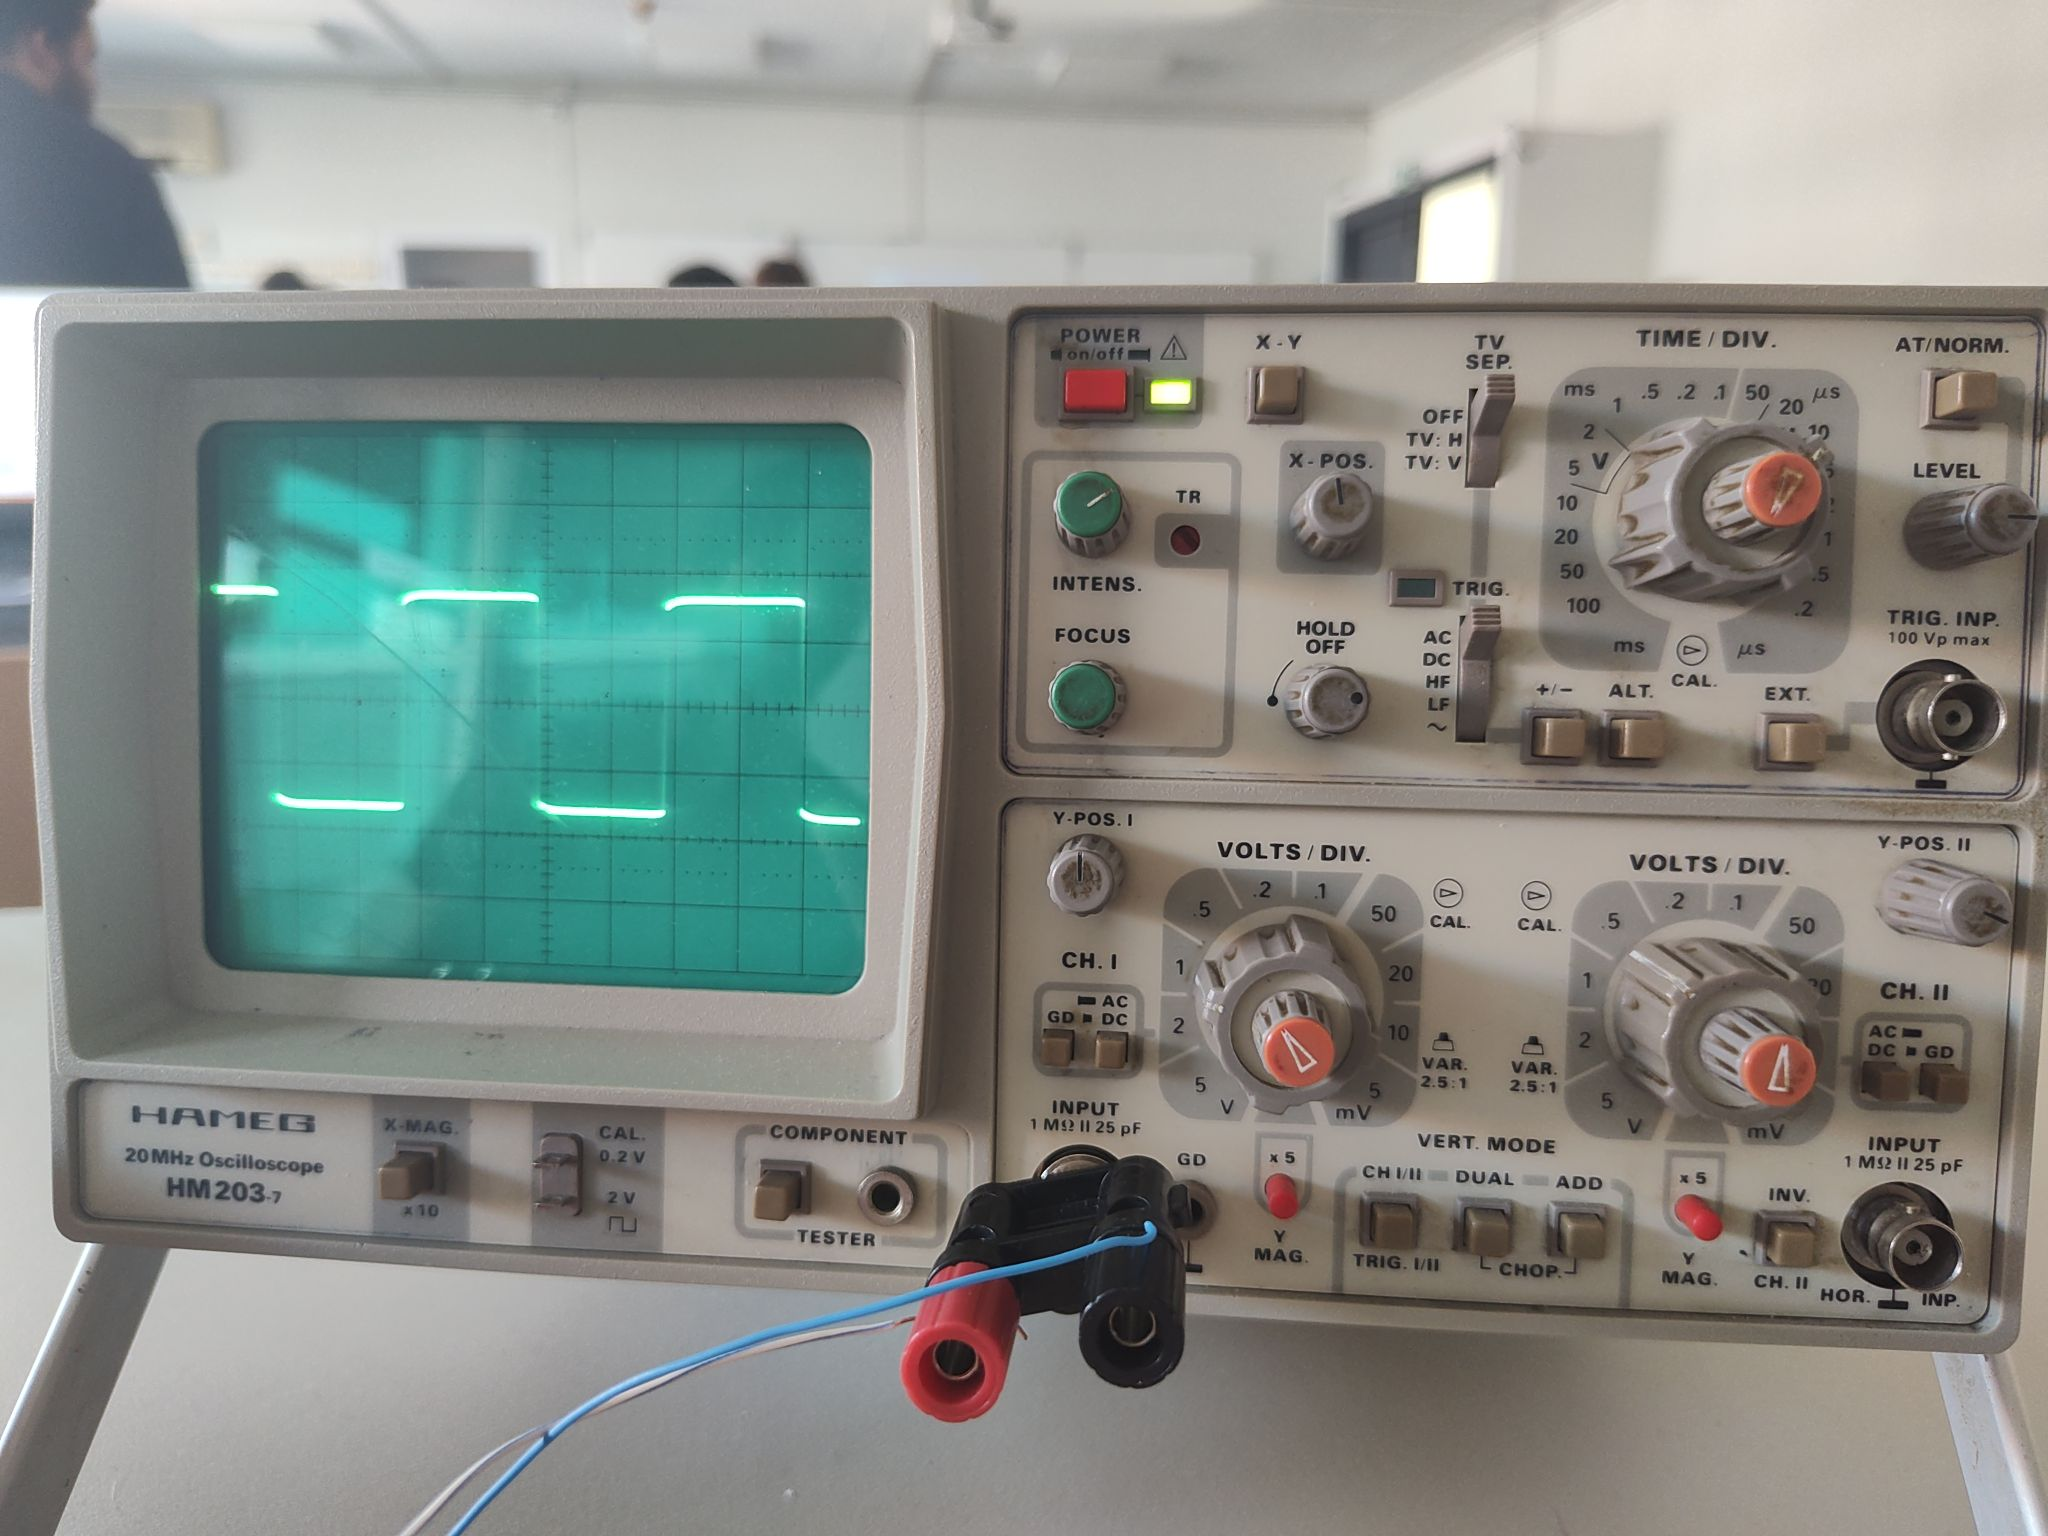
\includegraphics[width=\linewidth]{./res/square_real.jpg}
	\caption{Τετραγωνικό σήμα στον εργαστηριακό παλμογράφο.}
\end{figure}

\begin{figure}[H]
	\centering
	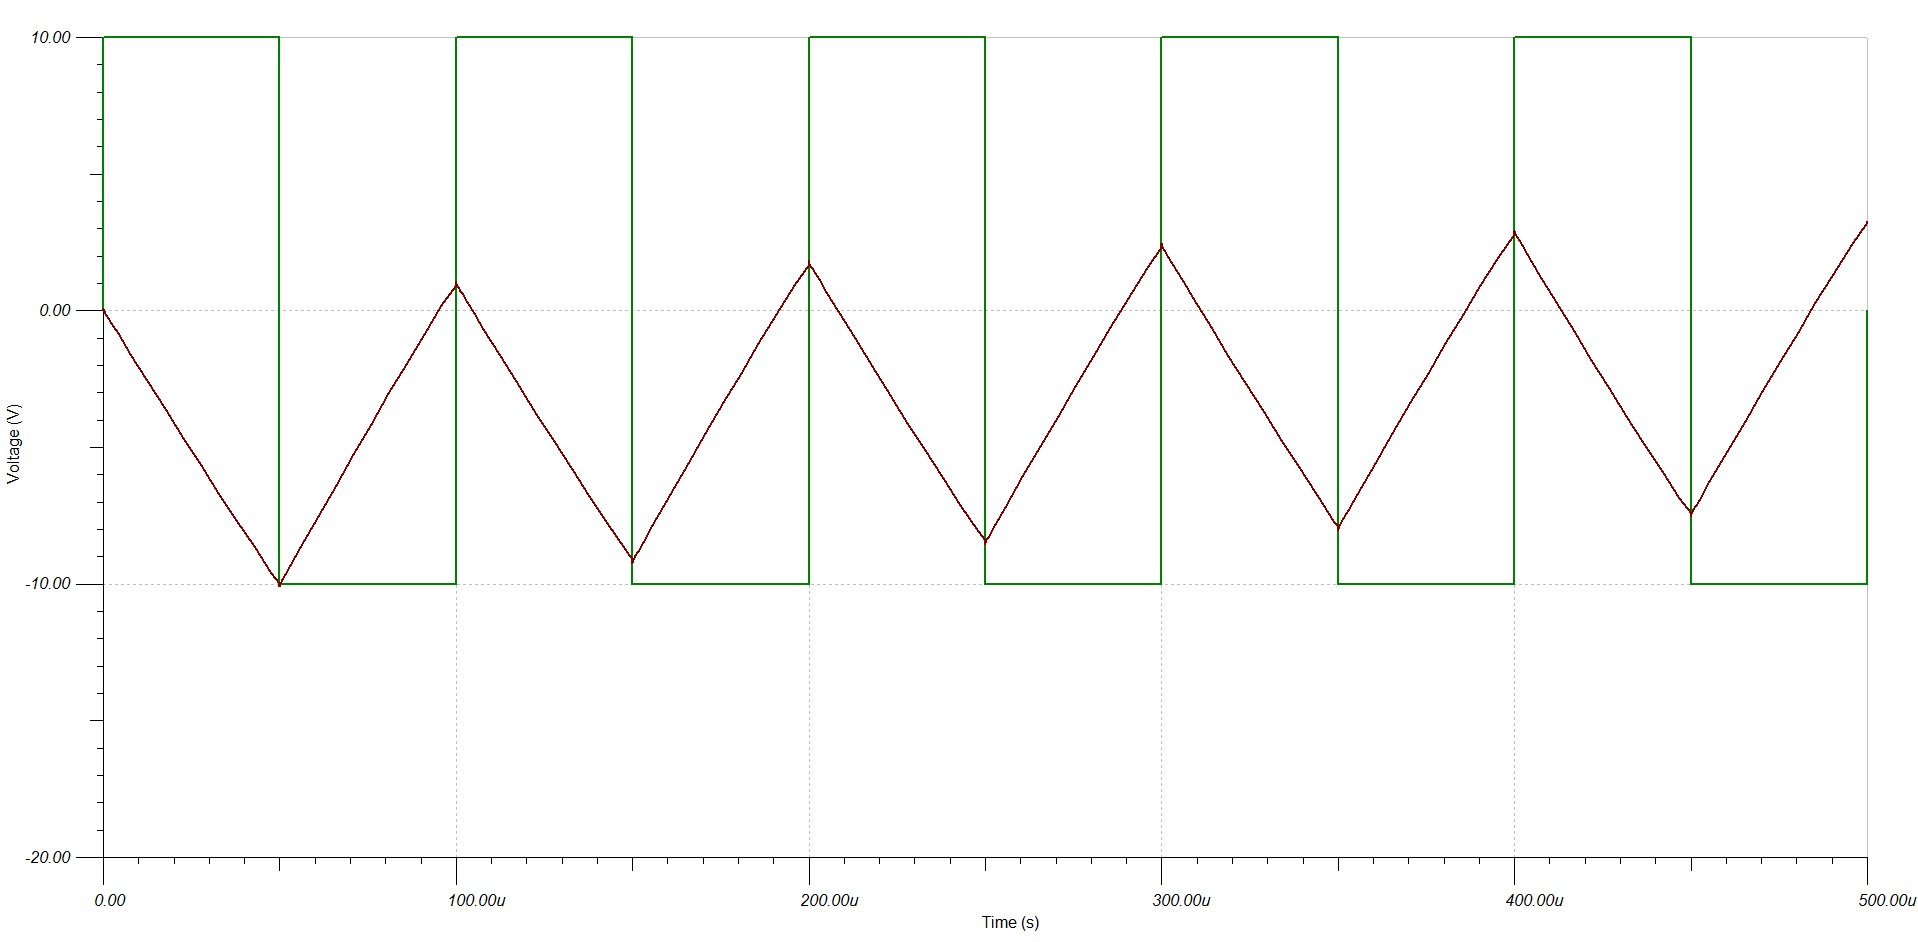
\includegraphics[width=\linewidth]{./res/square.jpg}
	\caption{Τετραγωνικό σήμα.}
\end{figure}

\subsection{Αύξηση τριγωνικής συχνότητας}

\begin{itemize}
	\item Για τριγωνική κυματομορφή εισόδου $7V_{pp}$, $\SI{400}{\hertz}$,
		αρχίστε να αυξάνετε την συχνότητα του σήματος έως ότου να
		παρατηρήσετε στην έξοδο του κυκλώματος την ύπαρξη τριγωνικής
		κυματομορφής Σημειώστε την πειραματικά μετρούμενη συχνότητα του
		κυκλώματος. Τι σχέση έχει η θεωρητική με την πρακτική συχνότητα
		$F_c$;
\end{itemize}

\begin{figure}[H]
	\centering
	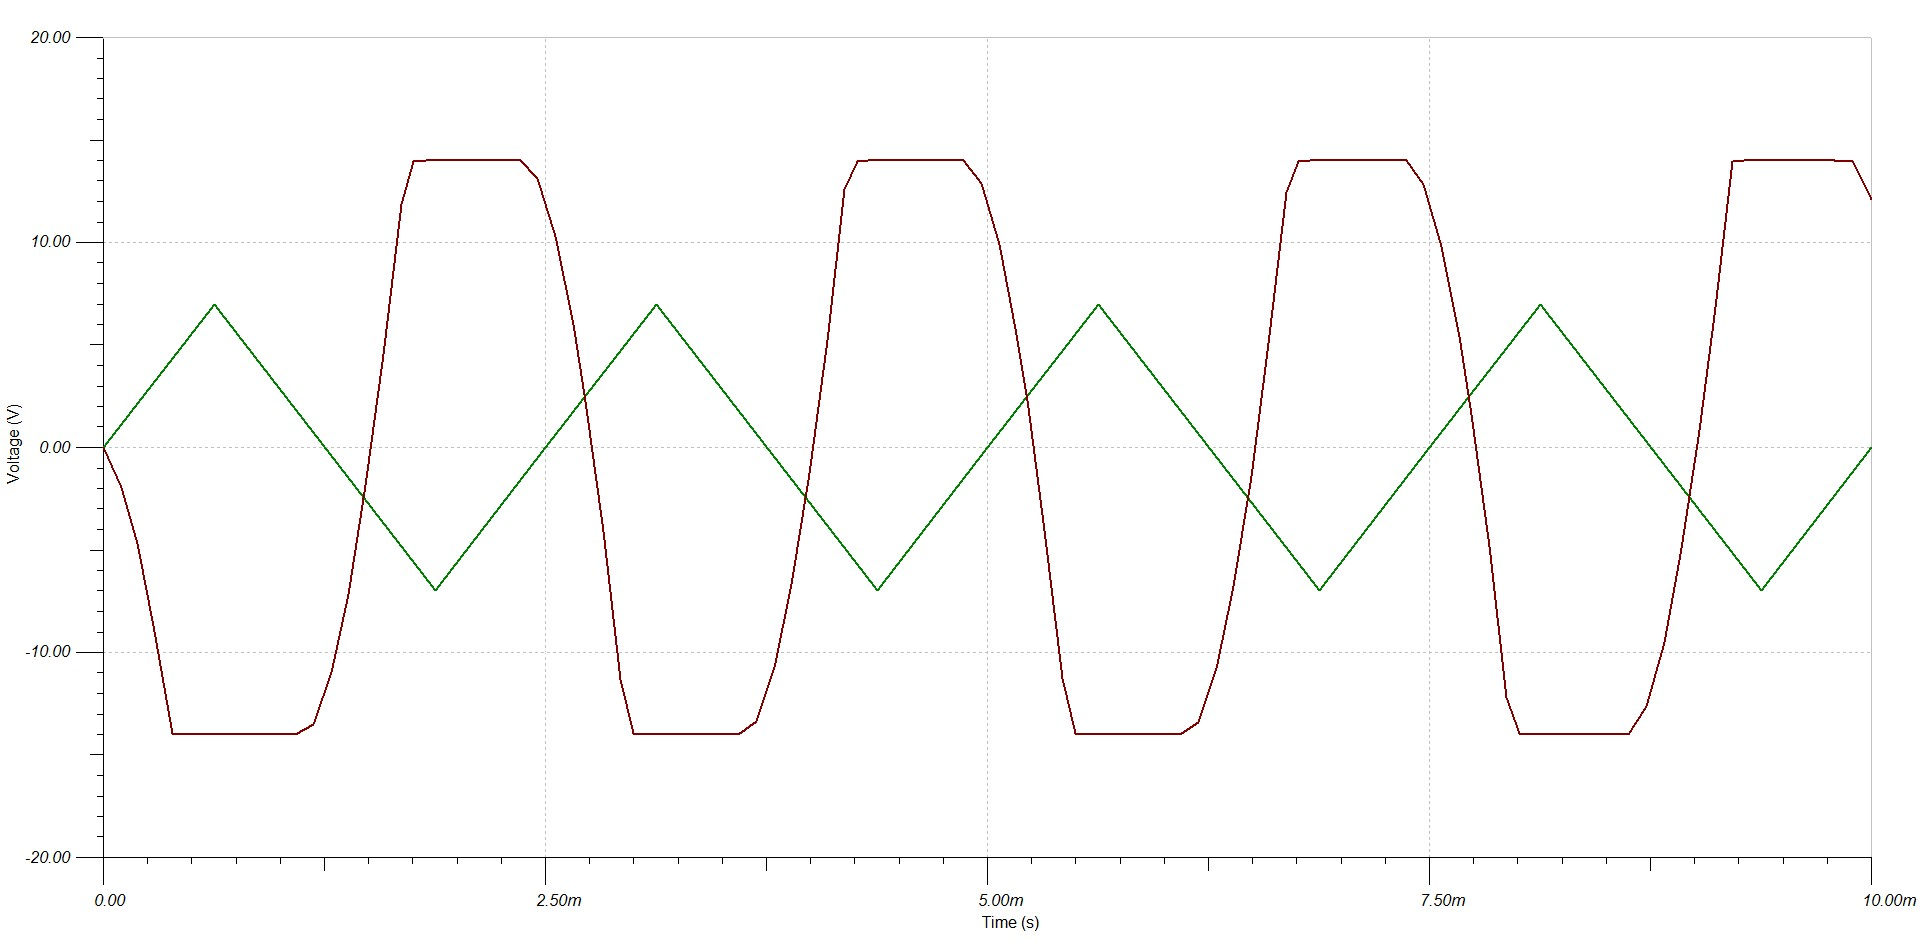
\includegraphics[width=\linewidth]{./res/triang_400hz.jpg}
	\caption{Τριγωνική συχνότητα $\SI{400}{\hertz}$}
\end{figure}

Μετά από πειραματισμό παρατήρησα ότι περίπου στα $\SI{2.5}{\kilo\hertz}$ η
έξοδος αρχίζει να γίνεται τριγωνικής μορφής, δηλαδή ο ολοκληρωτής λειτουργεί
σαν αναστρέφων Τ.Ε. Βλέπουμε ότι η πρακτική συχνότητα $\SI{2.5}{\kilo\hertz}$
είναι κοντά με την θεωρητική $F_c = \SI{3.3}{\kilo\hertz}$.

\begin{figure}[H]
	\centering
	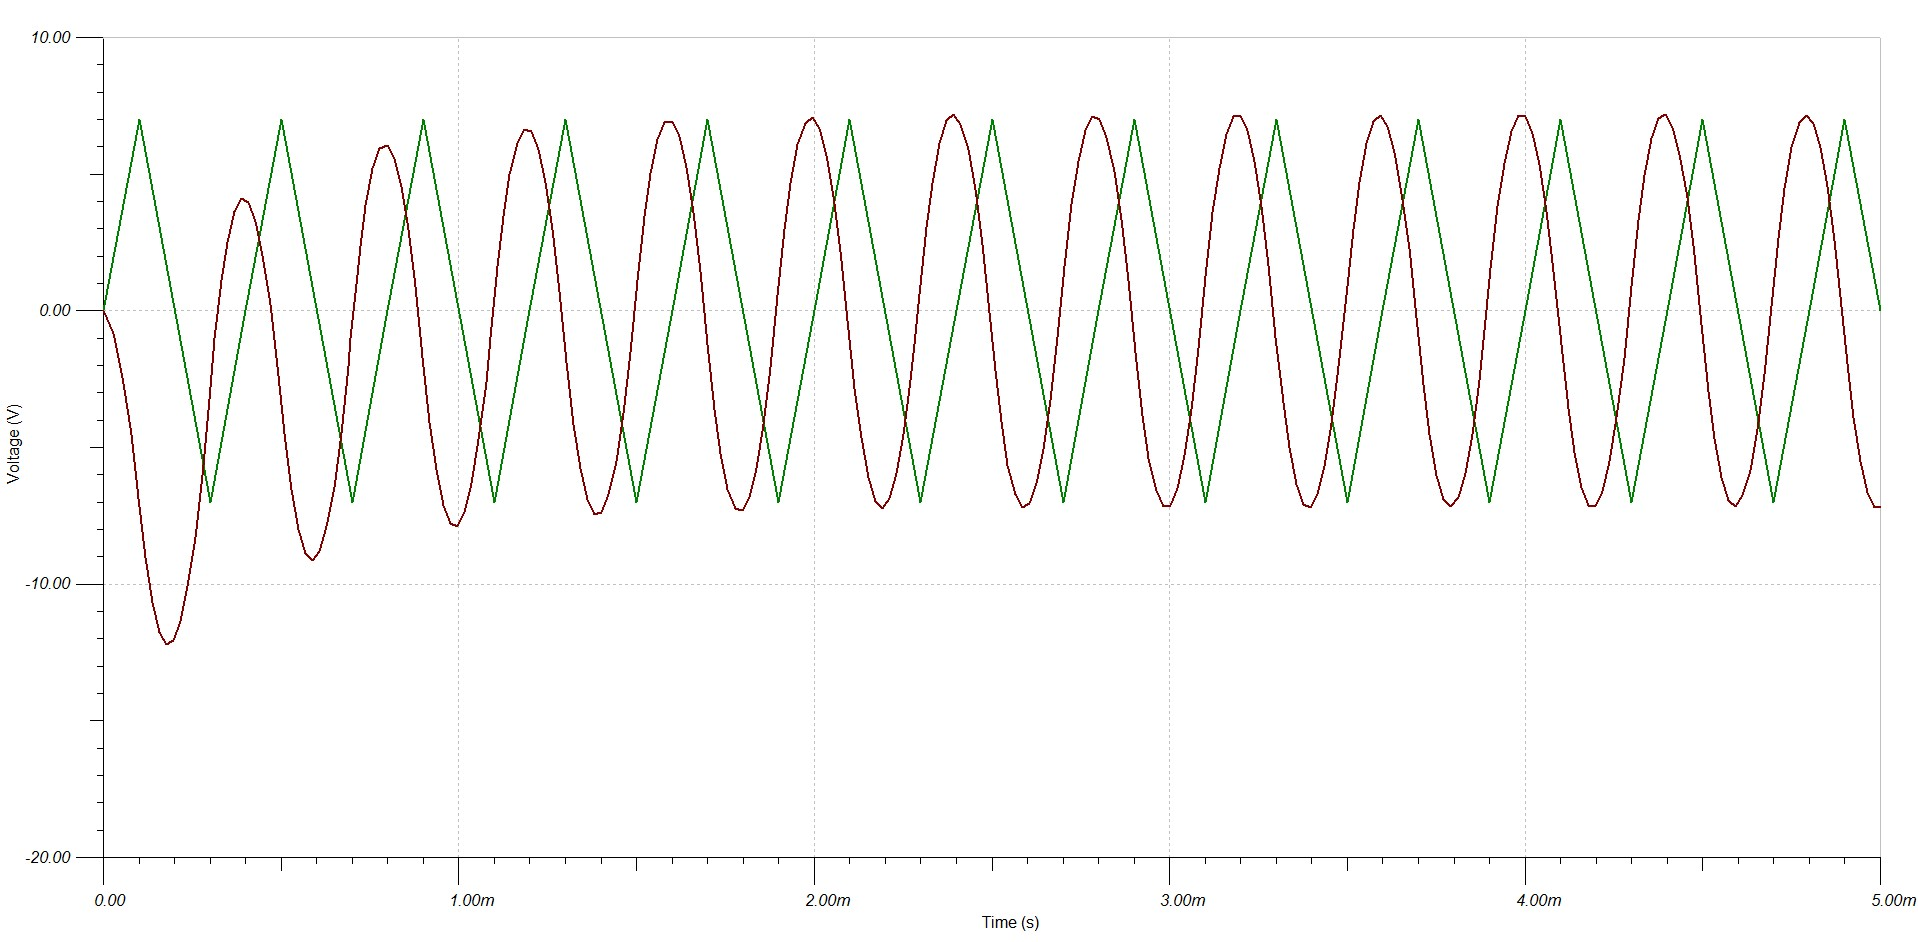
\includegraphics[width=\linewidth]{./res/triang_2.5khz.jpg}
	\caption{Τριγωνική συχνότητα $\SI{2.5}{\kilo\hertz}$}
\end{figure}

\section{Breadboard}

Η συνδεσμολογία έγινε στον χώρο του εργαστηρίου. Για την σύνδεση του Τ.Ε
χρησιμοποιούμε το pinout του Τ.Ε:

\begin{figure}[H]
	\centering
	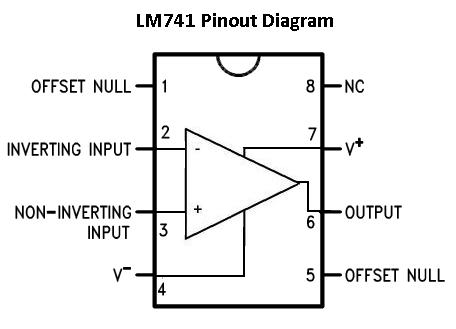
\includegraphics[width=\linewidth]{./res/opamp_pinout.jpg}
	\caption{Pinout Τ.Ε}
\end{figure}

\begin{figure}[H]
	\centering
	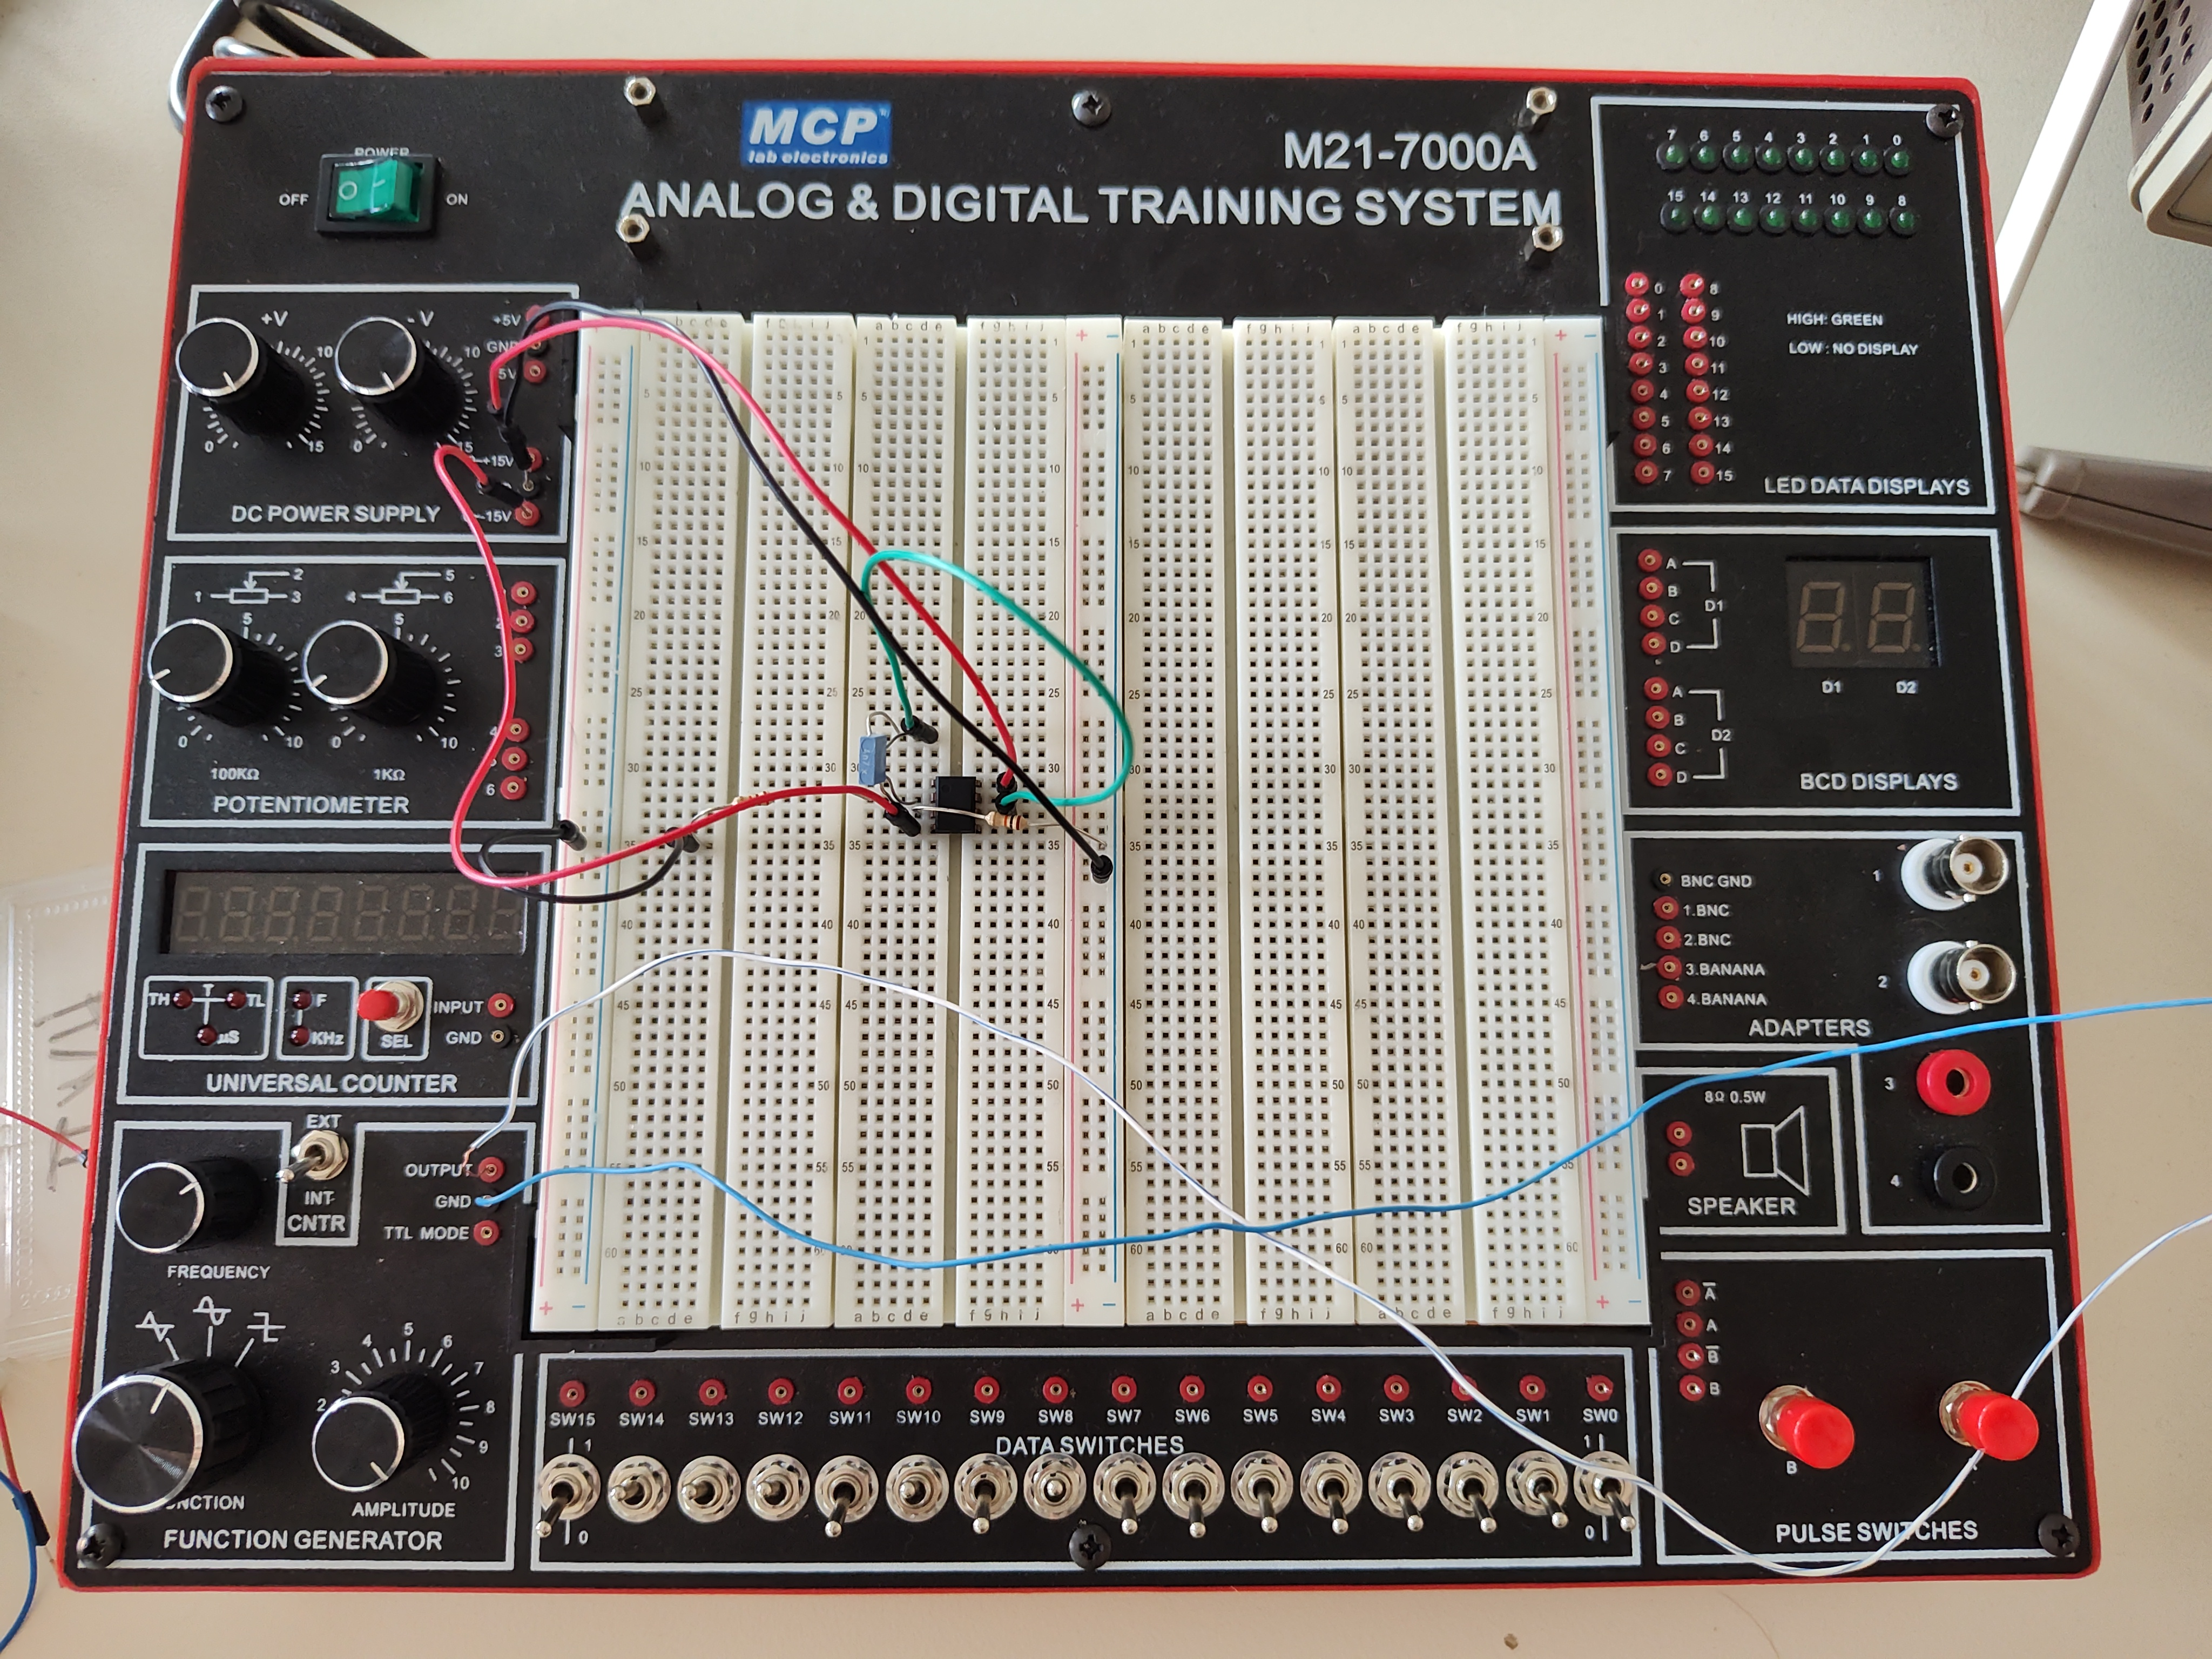
\includegraphics[width=\linewidth]{./res/breadboard.jpg}
\end{figure}

\end{document}
